%\documentclass[dvipdfmx]{beamer}
\documentclass{beamer}                   % lualatex の場合
\usepackage{mySld}

\begin{document}
\title[主記憶]{オペレーティングシステム\\第9章 メモリ割付け方式}
\date{}

\begin{frame}
  \titlepage
\end{frame}

%\section{}
%=========================================================================
%\begin{frame}
%  \frametitle{}
%\end{frame}

\section{固定区画方式}
%=========================================================================
\begin{frame}
  \frametitle{固定区画方式}
  \begin{center}
    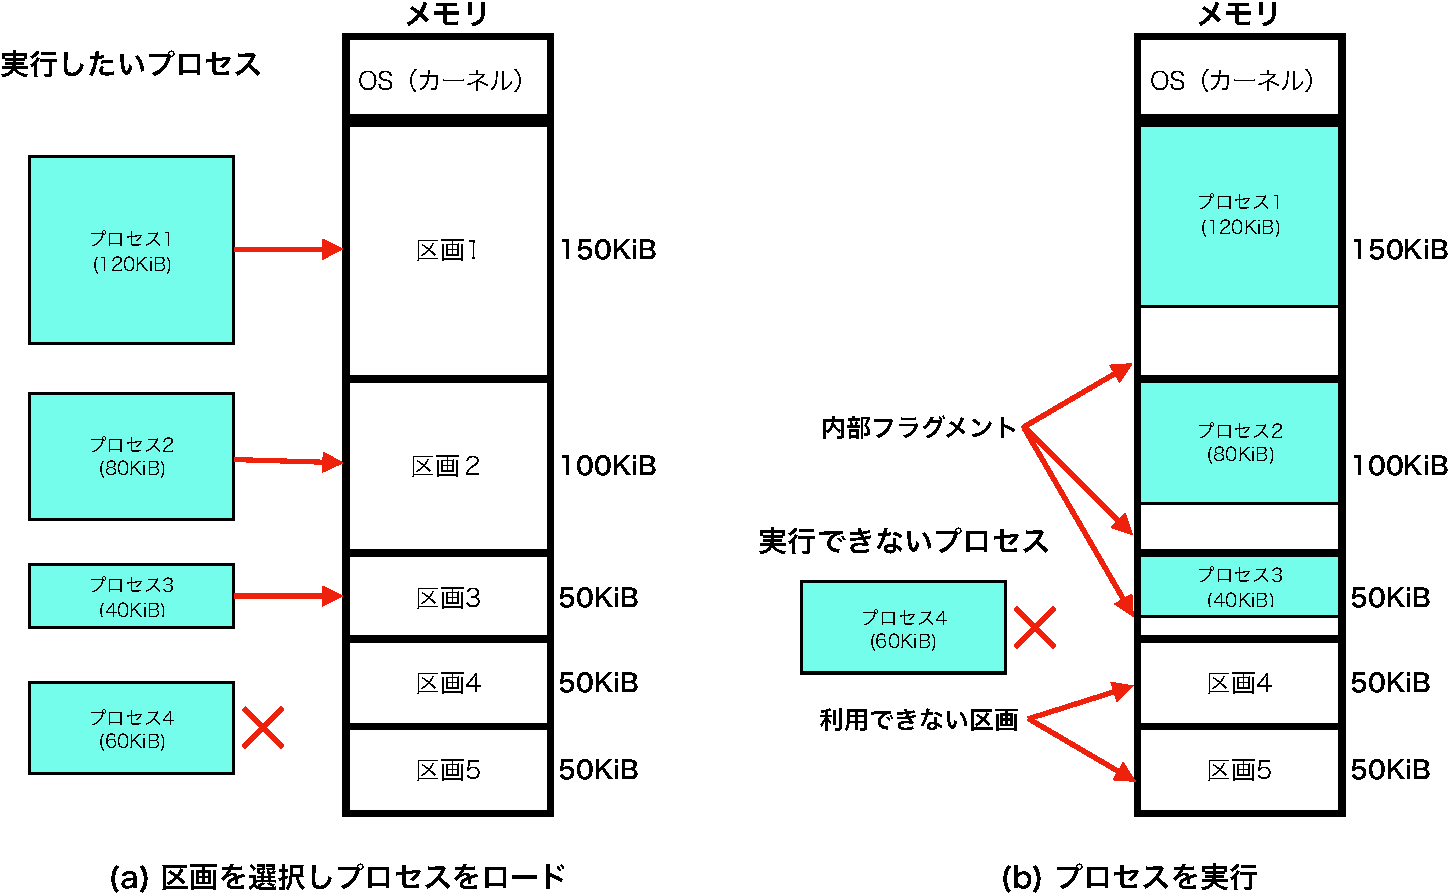
\includegraphics[scale=0.45]{Fig/fixedPartition-crop.pdf}\\
  \end{center}
  予めメモリを大小数種類の区画に分割しておく.
\end{frame}

%=========================================================================
\begin{frame}
  \frametitle{固定区画方式の特徴}
  \begin{enumerate}
  \item 空き領域の管理が容易である.
  \item 領域内部に無駄な領域({\bf 内部フラグメント})が生じる.
  \item 小さな領域が複数空いていても大きなプロセスは実行できない.
  \item 実行可能なプロセスのサイズに強い制約がある.\\
    (図の例では,151KiBのプロセスは実行できない.)
  \item 同時に実行できるプロセスの数に制約がある.\\
    (図の例では,同時に五つ以上のプロセスは実行できない.)
  \end{enumerate}
\end{frame}

\section{可変区画方式}
%=========================================================================
\begin{frame}
  \frametitle{可変区画方式}
  \begin{center}
    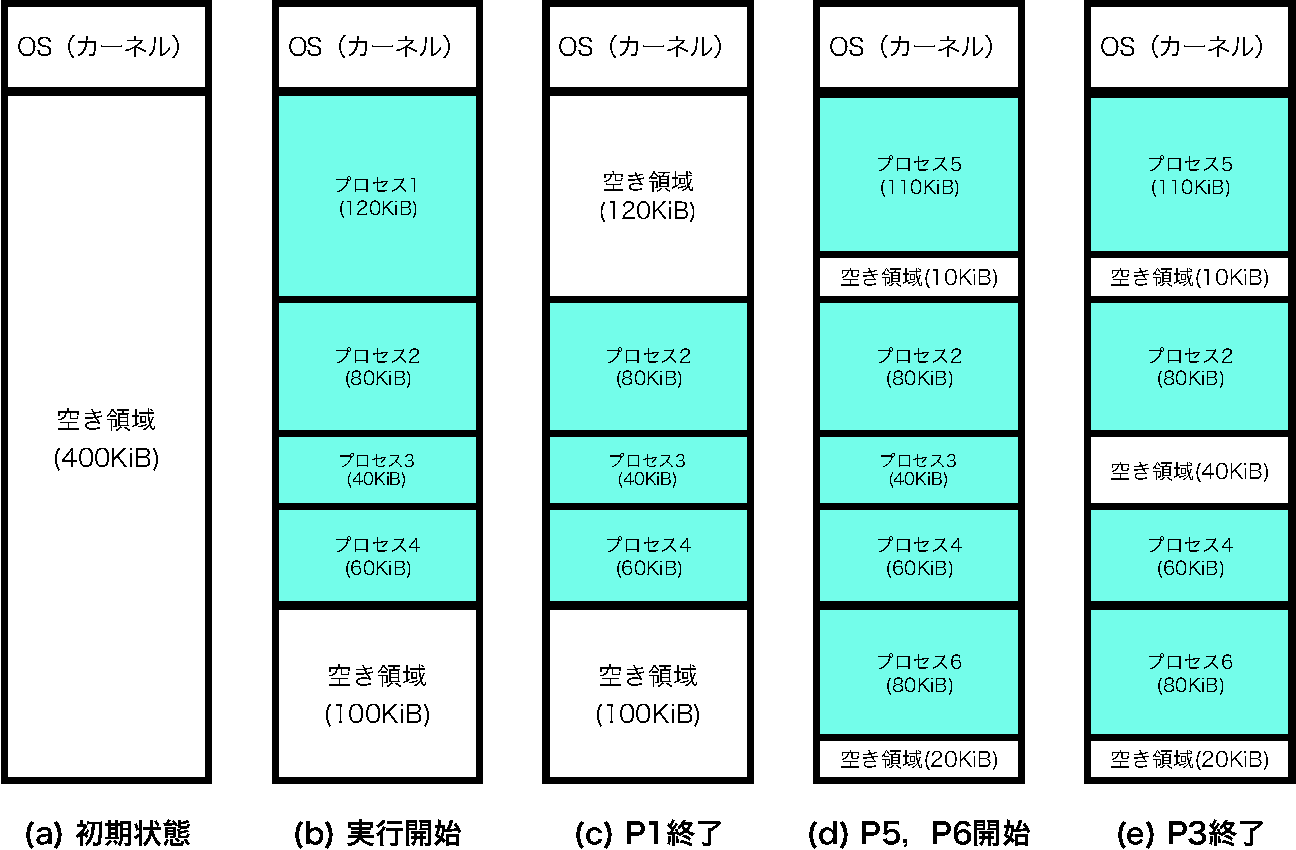
\includegraphics[scale=0.45]{Fig/variablePartition-crop.pdf}\\
  \end{center}
  必要に応じて空き領域から区画を作る.\\
  {\bf 外部フラグメント}が生じる.
\end{frame}

\section{可変区画方式の領域選択方式}
%=========================================================================
\begin{frame}
  \frametitle{可変区画方式の領域選択方式}
  \begin{center}
    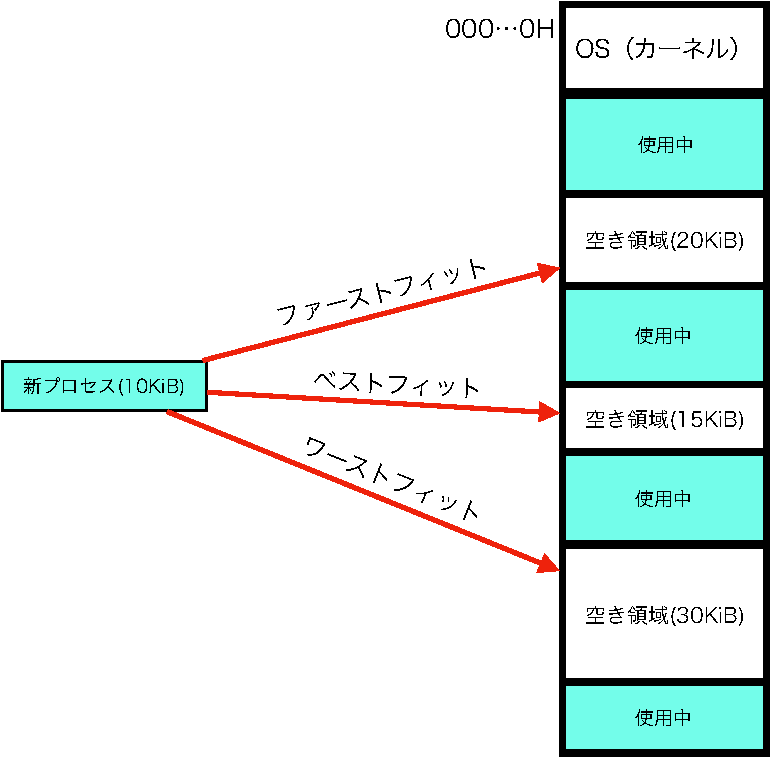
\includegraphics[scale=0.4]{Fig/firstBestWorstFit-crop.pdf}\\
  \end{center}
  \begin{itemize}
  \item ファーストフィット(first-fit)方式:アドレス順にさがす.
  \item ベストフィット(best-fit)方式:最小の領域を選択する.
  \item ワーストフィット(worst-fit)方式:最大の領域を選択する.
  \end{itemize}
\end{frame}

\section{空き領域の管理方式}
%=========================================================================
\begin{frame}
  \frametitle{空き領域の管理方式(ビットマップ方式)}
  どこに利用可能な空き領域があるかビットマップで管理する.
  \begin{center}
    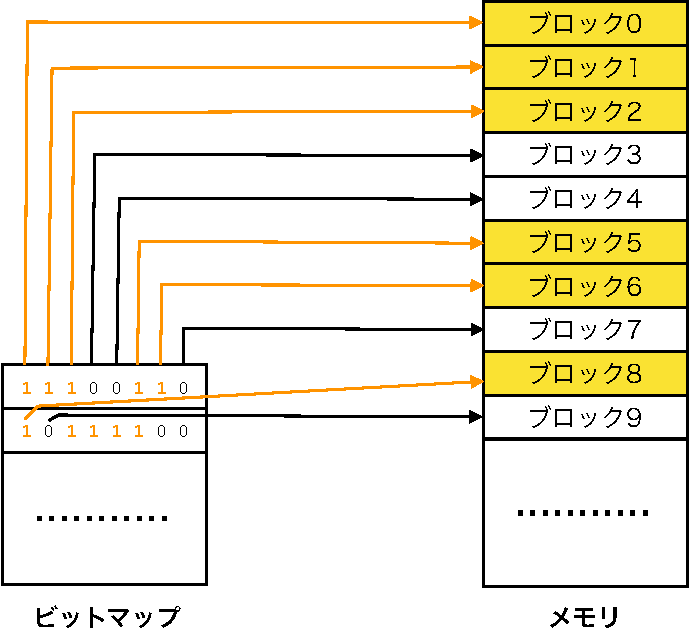
\includegraphics[scale=0.5]{Fig/bitMap-crop.pdf}\\
  \end{center}
  \begin{itemize}
  \item メモリを一定の大きさのブロックに分割する.
  \item ビットマップの1ビットが1ブロックに対応する.
  \end{itemize}
\end{frame}

%=========================================================================
\begin{frame}
  \frametitle{ビットマップの大きさ}
  ビットマップの大きさを計算してみる.
  \begin{itemize}
  \item メモリサイズ:8GiB
  \item ブロックサイズ:4KiB
  \item ブロック数:$8GiB \div 4KiB = (8\times 2^{30}) \div (4 \times 2^{10})
    = 2 \times 2^{20} = 2Mi$
  \item ビットマップのサイズ:$(2 \times 2^{20}) \div 8 = 2^{18} = 256KiB$
  \end{itemize}
  無視できるほど小さくはない.\\
  ビットマップを小さくするにはブロックサイズを大きくすればよい.\\
  内部フラグメントが大きくなる.
\end{frame}

%=========================================================================
\begin{frame}
  \frametitle{空き領域の管理方式(リスト方式)}
  空き領域をリストにして管理する.\\
  様々なサイズの空き領域が混在しても良い.
  \begin{center}
    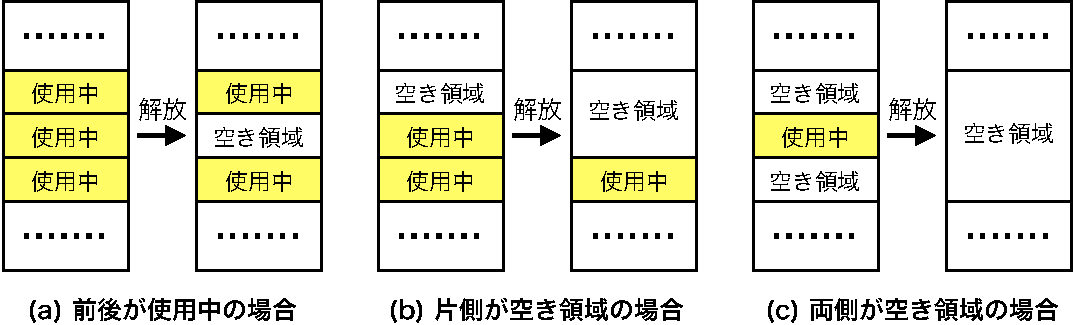
\includegraphics[scale=0.5]{Fig/memFree-crop.pdf}\\
  \end{center}
  使用中の領域が解放されると隣接する空き領域と合体させる.
\end{frame}

%=========================================================================
\begin{frame}
  \frametitle{空き領域リストのデータ構造}
  \begin{center}
    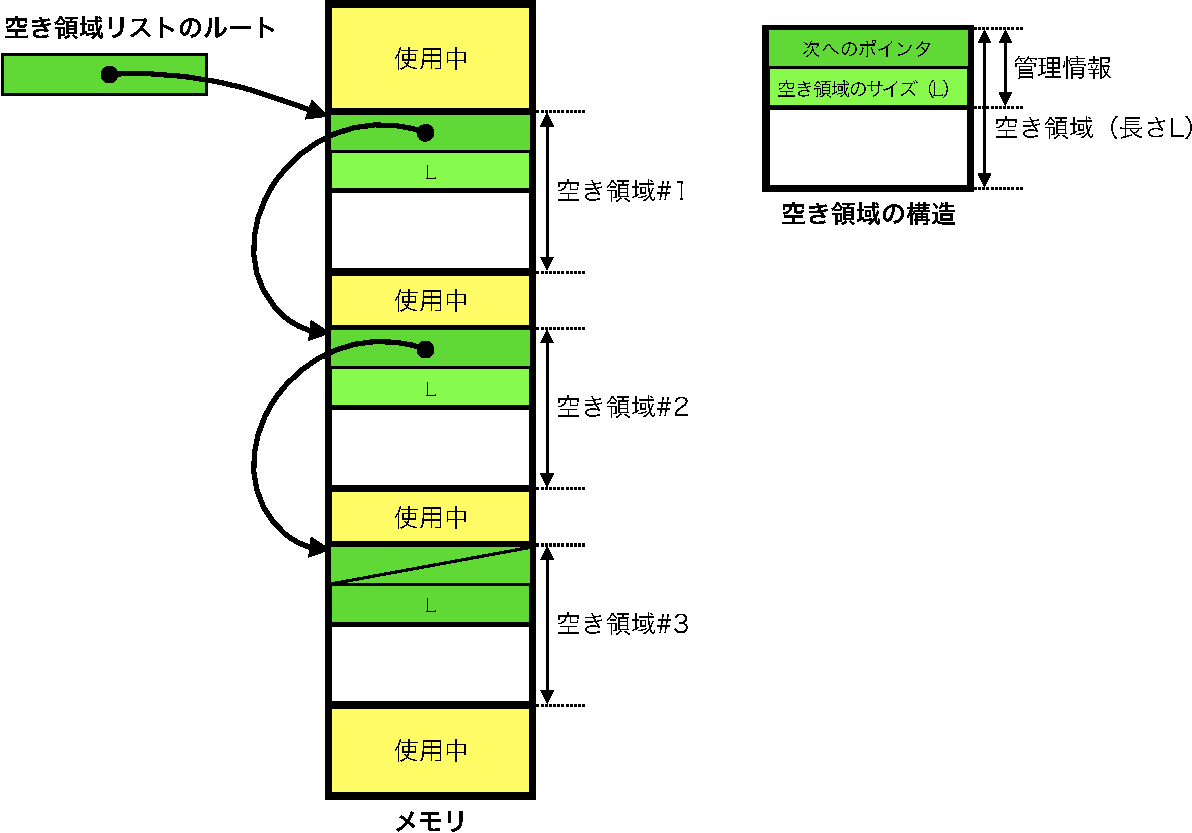
\includegraphics[scale=0.38]{Fig/linkedList-crop.pdf}\\
  \end{center}
  \begin{itemize}
    \item 空き領域の一部を管理データの格納に使用する.
    \item アドレス順のリストにして管理する.
    \item ファーストフィットの探索に都合が良い.
    \item 隣接領域との合体にも都合が良い.
  \end{itemize}
\end{frame}

%=========================================================================
\begin{frame}
  \frametitle{練習問題}
  可変区画方式で管理される100KiBの空き領域がある時,
  次の順序で領域の割付け解放を行った.
  ファーストフィット方式を用いた場合と
  ベストフィット方式を用いた場合について,
  実行後のメモリマップを図示しなさい.

  \begin{enumerate}
  \item[1] 30KiBの領域を割付け
  \item[2] 40KiBの領域を割付け
  \item[3] 20KiBの領域を割付け
  \item[4] 先程割付けた40KiBの領域を解放
  \item[5] 10KiBの領域を割付け
  \end{enumerate}
\end{frame}

\end{document}
